\textbf{write about how the programs interaction work}
\section{Programming in OpenCV and Unity}

In the end, the result should be a smoother experience than if only OpenCV was used.

Here is how we did stuff

What we did and why?

\section{Our own picture class}
\subsection{the idea of not using openCV}
\subsection{the pixel system}
\subsection{the functions}

\section{Config Background}
\subsection{Take Background picture}
wait until nothing moves:
	Threshold pixel value
	Threshold pixel amount
	Threshold picture amount
take picture
\subsection{find roi and enter and exit zone}
average brightest pixel in column for Roi
pixel for enter and exit

\section{The four in one function}
discard information that is not in the ROI(Make the pixels black that aren't used)
refresh(Open in openCV, write to write to pointer system)
background subtraction(compare the current picture to the background)
threshold pixel values and set to true(255) or false(0)- outcome binary picture

\section{Morphology}
Closing
	erode
	dilate
	
\section{persons}
why first old and then new
\subsection{find old person}
loop trough persons
when position is set:
	first look at the position where the person would be when it would move with the same speed as captured in the last frame.
	second look if the position has not changed meaning that the person stoped up.
	third go from the point between the two previously check points and move to the sides until the max distance to move i reached
	if the person is not found after this it can be assumed that the person is either gone out of the picture or is occlude by another person. To check if the person is exited, the program checks if the person is close enough to the edge of the picture so it could have exit. If the person is not close enough to the border of the  picture the program will try to find another person that is close enough that it could occlude the person we are looking at.  This is done in the same way as the search for a person in the first place.
	
\subsection{find new person}

When all persons are found again the program looks for new persons. To make the program more efficient it loops not through all pixels but through the ones where it is most likely that a person could enter to the picture. Because of the placement of the camera the persons can just enter from left and right so we can limit the enter and exit zone to the most left and most right pixels. 

\subsection{the awesome move vector reconfig}

\section{Using Unity to handle the graphical output}
After doing the initial prototype, the group realized that for it would be difficult to use OpenCV to both extract the data from the camera and display it in some kind of graphical way. Since the program has to loop through a lot of data continuously, there was little resources left for it to actually display the result in an interesting way without lagging behind. First the group thought about using multiple threads running in the program, but even then it would be hard to display more sophisticated graphics. OpenCV is not meant as a tool to display graphics, but more to for the analyzing/extracting part.

Then the group came up with the idea of using the Unity game engine to display the graphics based on the data from OpenCV. This had the added bonus of being able to use elements such as particle effects, physics and sound. Since some group members already had experience with the Unity, it seemed a good choice. The only concern was how to send the data from OpenCV to Unity. OpenCV uses C++, while Unity uses \texttt{C\#}, JavaScript or Boo as scripting languages. Even though there are various APIs to get OpenCV and Unity communicate, it was decided for a much simpler approach where OpenCV would copy some position data into a text file that Unity would read.

\subsection{Heysa}
Different possibilities (pros and cons)
Show code and describe features
Test individual features - e.g. why did we use threshold value X instead of Y?

OpenCV
Using Picture struct
ROI
Using ClipBoard Manager
Unity - uses time of day to change stuff

\begin{lstlisting}
Mat MeanFilter(Mat input)
{
	// 5x5 kernel

	// Make a temporary clone of the input image
	Mat mean = input.clone();

	int jegErSej = 42;
}
\end{lstlisting}

\subsection{Using Unity to display the characters}
The Unity game engine is typically used to make 3D games, but it is still possible to make programs in 2D, using 2D sprites/textures and an orthographic camera that doesn't display depth.

The scene used for the game is quite simple. As shown in figure XX, it consists of a background image showing mountains. To achieve a more dynamic look, a couple of elements are added to make the whole scene spring to life.

First there are are a collection of Christmas trees with some Christmas balls and bells hanging on top. Using built-in physics in Unity, these bouncy back and forth, simulating a wind effect. Along with this is the falling snow, which is made as an particle system in Unity. This ensures that even when there are nobody in front of the camera, the program still feels alive.

\subsection{Time manager and Santa Claus}
As mentioned in chapter \ref{hjoerring}, the library is build on the theme of serendipity, e.g. to surprise and be new. When making the program, the group had an idea about having it change depending on the time of the day. Using the clock in Windows, the program could do something different at different times.

In the program, the a sun will gradually rise as time goes, as well as the light will become brighter/dimmer, just as it is happening outside. Figures \ref{fig:time1}, \ref{fig:time2} and \ref{fig:time3} illustrate this.

\begin{figure}[htbp]\centering
	\begin{minipage}[b]{0.3\textwidth}\centering
		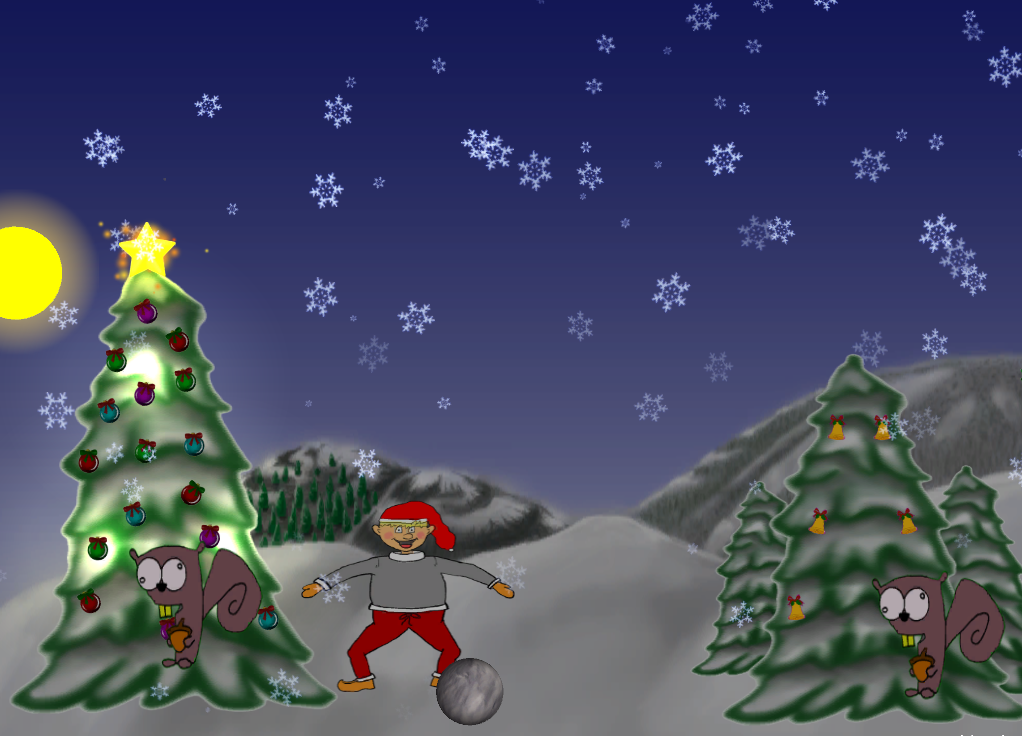
\includegraphics[width=1.00\textwidth]{Pictures/Design/time1.png} %Venstre billede
	\end{minipage}\hfill
	\begin{minipage}[b]{0.3\textwidth}\centering
		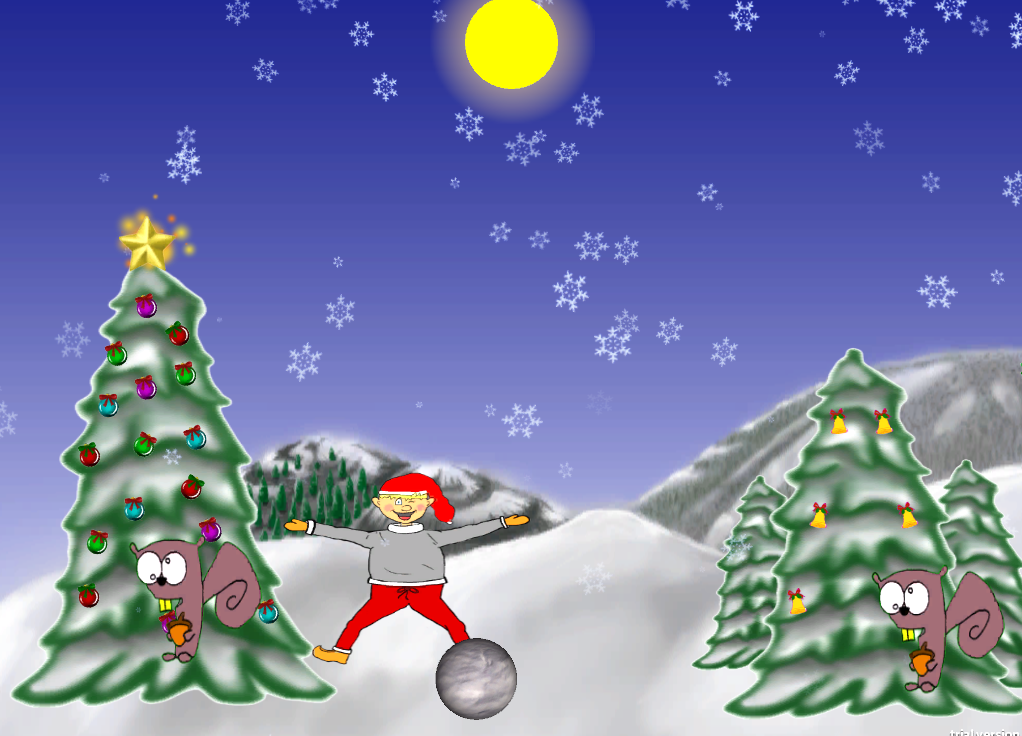
\includegraphics[width=1.00\textwidth]{Pictures/Design/time2.png} %Venstre billede
	\end{minipage}\hfill	
	\begin{minipage}[b]{0.3\textwidth}\centering
		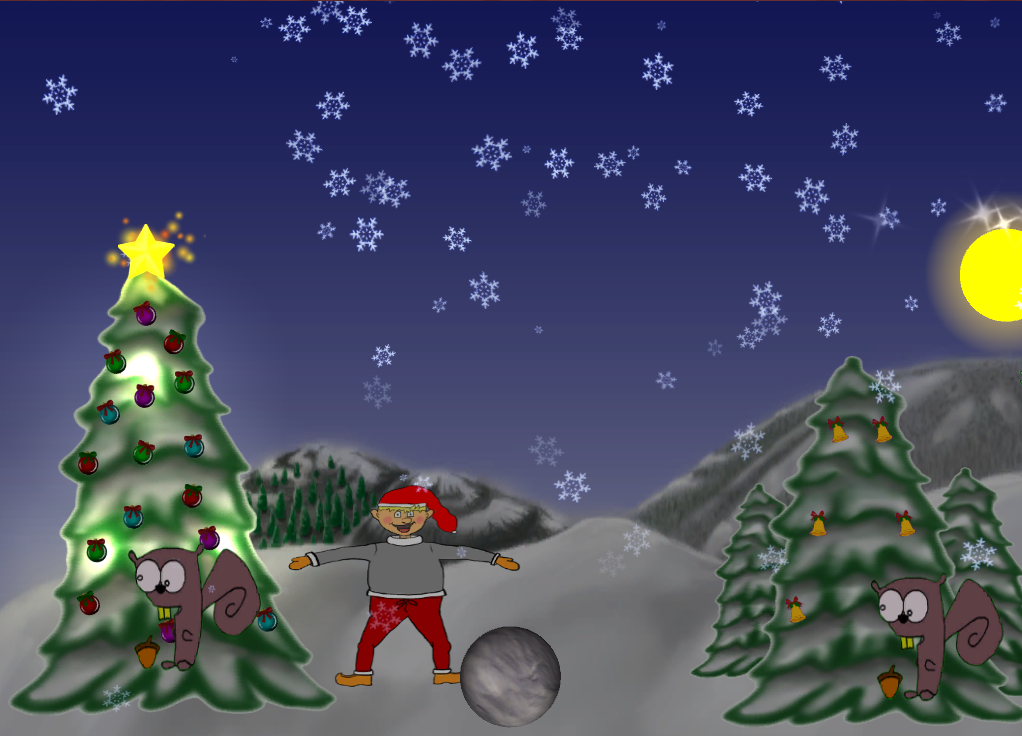
\includegraphics[width=1.00\textwidth]{Pictures/Design/time3.png} %Højre billede
	\end{minipage}\\ %Captions and labels
	\begin{minipage}[t]{0.3\textwidth}
		\caption{Morning.} %Venstre caption og label
		\label{fig:time1}
	\end{minipage}\hfill
	\begin{minipage}[t]{0.3\textwidth}
		\caption{Noon.} %Venstre caption og label
		\label{fig:time2}
	\end{minipage}\hfill	
	\begin{minipage}[t]{0.3\textwidth}
		\caption{Evening.} %Højre caption og label
		\label{fig:time3}
	\end{minipage}
\end{figure}

Another aspect is Santa Claus who will come at a randomly chosen time (see figure \ref{fig:santa}. When he arrives, jingle bell sounds play, as well as his iconic "ho ho ho". Santa will then drop packages that can be interacted with. This happens by moving into the objects, pushing them with the physics system in Unity. It should be noted that Santa doesn't come too often, since it would disturb other visitors at the library. In average, Santa Claus arrives once an hour.

\begin{figure}[htbp]
\centering
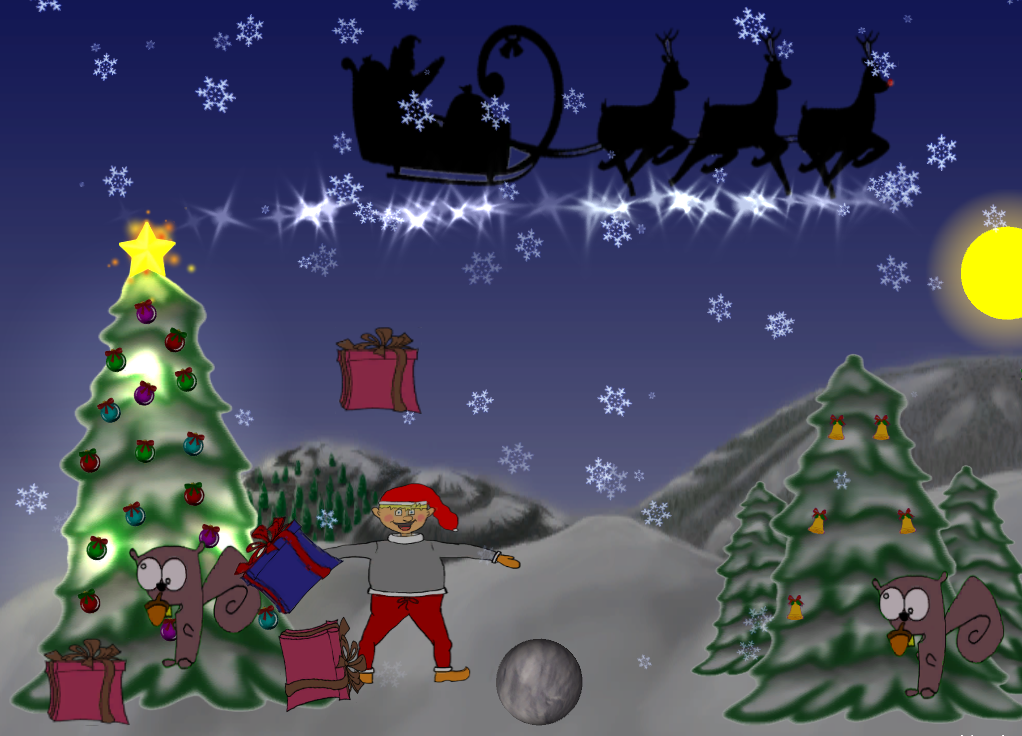
\includegraphics[width=0.90\textwidth]{Pictures/Design/santa.png}
\caption{Santa Claus comes at random times and drop presents. These can be pushed by the characters. They disappear after some time.}
\label{fig:santa}
\end{figure}

\subsection{Snow ball}
To get a little more interaction, a snow ball is placed in the scene. This can be pushed around by the characters, and it will gradually grow bigger and bigger until it at some time explodes and disappear for a short while.

One thing we needed to have in mind was the light setting. On a computer screen the image can be really bright and really dark, but on a canvas and a projector it is not easy to see a dark image. Therefore the brightness level was set a little higher than normal, so it would still be possible to see it properly on the canvas.

\begin{figure}[htbp]
\centering
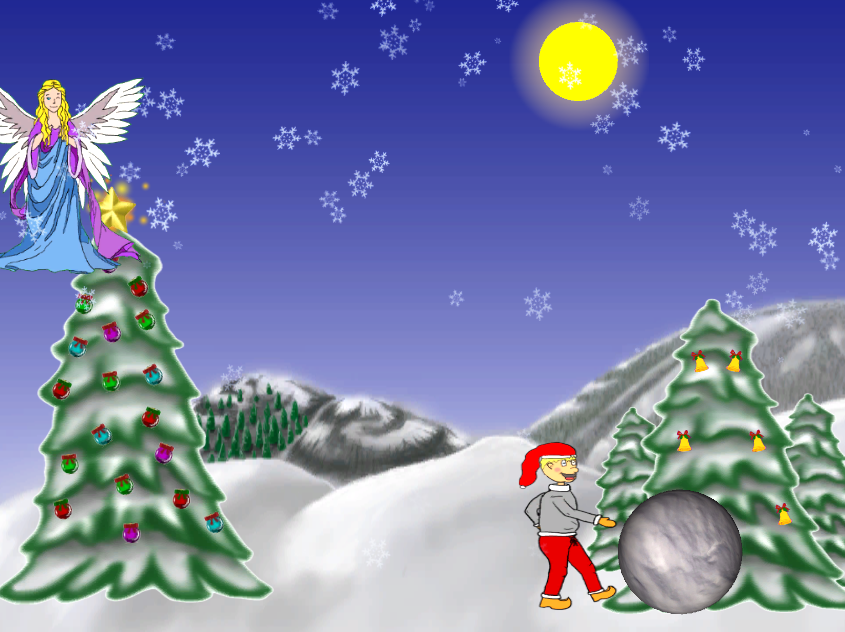
\includegraphics[width=0.90\textwidth]{Pictures/Design/pushing_snowball.png}
\caption{The characters can push the snowball to make it grow. When it becomes big enough, it explodes into colorful fireworks.}
\label{fig:santa}
\end{figure}

\section{Conclusion and limitations}
During the setup at the library multiple things were learned.

\subsection{Use of LED stripes}
\subsection{Santa Claus ho ho sound}
\subsection{Shadows on canvas}
\subsection{Need sound to draw attention}
\subsection{People walking too fast}
\subsection{Camera not steady}

